\documentclass[conference]{IEEEtran}
\IEEEoverridecommandlockouts
% The preceding line is only needed to identify funding in the first footnote. If that is unneeded, please comment it out.
\usepackage[T5]{fontenc}
\usepackage[utf8]{inputenc}
\usepackage{vietnam}

% Restore English labels for IEEEtran layout at document start
\makeatletter
\AtBeginDocument{
  \def\tablename{Table}
  \def\figurename{Figure}
  \def\abstractname{Abstract}
  \def\refname{References}
  \@ifundefined{captionsvietnamese}{}{
    \addto\captionsvietnamese{
      \def\tablename{Table}
      \def\figurename{Figure}
      \def\abstractname{Abstract}
      \def\refname{References}
    }
  }
  \@ifundefined{captionsvietnam}{}{
    \addto\captionsvietnam{
      \def\tablename{Table}
      \def\figurename{Figure}
      \def\abstractname{Abstract}
      \def\refname{References}
    }
  }
}
\makeatother

% Float parameters to prevent half-empty pages and force better distribution
\renewcommand{\topfraction}{0.95}
\renewcommand{\bottomfraction}{0.95}
\renewcommand{\textfraction}{0.05}
\renewcommand{\floatpagefraction}{0.90}
\setcounter{topnumber}{3}
\setcounter{bottomnumber}{3}
\setcounter{totalnumber}{6}

% Prevent stretchable vertical space on float pages
\makeatletter
\setlength{\@fptop}{0pt}
\setlength{\@fpsep}{12pt}
\setlength{\@fpbot}{0pt plus 1fil}
\makeatother

\usepackage{cite}
\usepackage{dblfloatfix}   % Fix table*/figure* placement in two-column mode
\usepackage{afterpage}     % Flush pending floats cleanly before a section



\usepackage{amsmath,amssymb,amsfonts}
\usepackage{algorithmic}
\usepackage{graphicx}
\usepackage{textcomp}
\usepackage{xcolor}
\usepackage{booktabs}
\usepackage{url}
\usepackage{hyperref}
\usepackage{algorithm}




\def\BibTeX{{\rm B\kern-.05em{\sc i\kern-.025em b}\kern-.08em
    T\kern-.1667em\lower.7ex\hbox{E}\kern-.125emX}}
    
\begin{document}

\title{Vietnamese Clickbait Detection and Explanation Using Fine-Tuned PhoBERT with Linguistic Feature Fusion and RAG\\
}

\author{\IEEEauthorblockN{Huynh Tran Khai Hoang}
\IEEEauthorblockA{\textit{Department of Computer Science} \\
\textit{FPT University}\\
Da Nang, Vietnam \\
hoanghtkh180321@fpt.edu.vn}
\and
\IEEEauthorblockN{Nguyen Minh Duy}
\IEEEauthorblockA{\textit{Department of Computer Science} \\
\textit{FPT University}\\
Da Nang, Vietnam \\
duynm180425@fpt.edu.vn}
}

\maketitle

\begin{abstract}
The rapid growth of online journalism in Vietnam has led to a proliferation of clickbait—headlines designed to attract clicks by exaggerating, sensationalizing, or withholding critical information. While clickbait detection has been studied extensively in English, research in Vietnamese remains constrained by linguistic challenges and a lack of unified datasets. In this paper, we propose a comprehensive, hybrid framework for Vietnamese clickbait detection, explanation, and rewriting using the newly released ViClickbait-2025 dataset. Our method fine-tunes PhoBERT, a state-of-the-art pre-trained language model optimized for Vietnamese, and fuses its deep contextual embeddings with seven hand-crafted surface linguistic features (including length, punctuation, and semantic markers). Furthermore, we address the lack of interpretability in existing classification models by proposing a Retrieval-Augmented Generation (RAG) pipeline. When a headline is classified as clickbait, the system retrieves the article's lead paragraph from a database and utilizes a Large Language Model (LLM) to generate a natural language explanation of the clickbait nature and propose an objective, factual alternative headline. Experimental results demonstrate that our proposed PhoBERT with Feature Fusion model achieves a Macro F1-score of $79.83\%$ and Accuracy of $82.46\%$, outperforming both standard TF-IDF+SVM and PhoBERT-only baselines. Automatic evaluation of the RAG rewriting component yields a ROUGE-L score of $44.84\%$ and ROUGE-1 of $56.19\%$, indicating high alignment with human factual reference titles and significant potential for enhancing information trust in Vietnamese digital media.
\end{abstract}

\begin{IEEEkeywords}
Clickbait Detection, PhoBERT, Feature Fusion, Retrieval-Augmented Generation (RAG), Vietnamese Natural Language Processing
\end{IEEEkeywords}

\section{Introduction}
Clickbait has become a dominant phenomenon in online news media, where publishers craft enticing, sensational, or misleading headlines to lure readers into clicking hyperlinks. This practice is driven by the ad-revenue model of digital publishing, which incentivizes click rates over content quality. Clickbait headlines typically employ stylistic devices such as curiosity gaps, exaggerated emotional appeal, and ambiguous referencing. While clickbait increases page views in the short term, it deteriorates user experience, spreads misinformation, and erodes public trust in digital journalism.

Detecting clickbait is a challenging task because it requires understanding the subtle boundaries between engaging writing and deliberate deception. In Vietnamese, this challenge is compounded by specific linguistic traits, such as word segmentation ambiguity, heavy use of tone markers, and complex honorifics. While deep learning models like BERT and RoBERTa have revolutionized clickbait detection globally, their direct application to Vietnamese text is sub-optimal. Pre-trained language models specific to Vietnamese, such as PhoBERT~\cite{nguyen2020phobert}, have shown superior performance in localized NLP tasks but remain under-explored for clickbait detection.

Moreover, existing clickbait detection systems function primarily as black-box classifiers. They output a binary label (``clickbait'' or ``non-clickbait'') without explaining why a headline is manipulative. This lack of transparency limits their utility for end-users, who remain uninformed about the nature of the exaggeration, and for editors, who need assistance in rewriting headlines to meet journalistic standards.

To address these limitations, this study proposes a complete framework for Vietnamese clickbait detection and explanation. Our core contributions are:
\begin{itemize}
    \item We design a hybrid neural classifier that integrates the deep semantic representations of PhoBERT with seven hand-crafted surface linguistic features designed to capture specific Vietnamese clickbait patterns.
    \item We present an interpretable Retrieval-Augmented Generation (RAG) pipeline that retrieves the factual lead paragraph of the corresponding article and generates natural language explanations detailing why the headline was flagged as clickbait.
    \item We utilize the RAG model to automatically rewrite clickbait headlines into objective, neutral, and informative titles.
    \item We conduct a comprehensive evaluation of both the classification and generation tasks using the ViClickbait-2025 dataset, establishing new performance benchmarks.
\end{itemize}

\section{Related Work}
\subsection{Clickbait Detection}
Early research on clickbait detection was centered on manual feature engineering paired with classical machine learning classifiers. Chakraborty et al.~\cite{chakraborty2016stop} extracted stylistic, punctuation, and part-of-speech patterns to train Support Vector Machines (SVM)~\cite{cortes1995svm} and Decision Trees for text categorization~\cite{joachims1998text}. Potthast et al.~\cite{potthast2016clickbait, potthast2018crowdsourcing} examined clickbait patterns on Twitter, identifying that informality, readability scores, and character-level n-grams are strong predictors of clickbait behavior. Biyani et al.~\cite{biyani2016clickbait} explored article informality and styling cues to separate clickbait from factual content in news streams, while Thomas and Warsi~\cite{thomas2017clickbait} proposed document-level features to represent clickbait structure.

With the emergence of deep learning, neural models replaced manual feature extraction. Agrawal~\cite{agrawal2016clickbait} and Dong et al.~\cite{dong2019deep} demonstrated the utility of Convolutional Neural Networks (CNNs) and recurrent architectures (LSTMs, GRUs) in automatically learning compositional word representations. Zhou~\cite{zhou2017clickbait} leveraged self-attention mechanisms~\cite{vaswani2017attention} over bi-directional recurrent architectures to capture distant word dependencies in headlines. In recent years, pre-trained transformer language models such as BERT~\cite{devlin2019bert} and RoBERTa~\cite{liu2019roberta} have been fine-tuned for clickbait classification, setting state-of-the-art benchmarks on public datasets. The transition from feature engineering to pre-trained representation tuning was studied in detail by Peters et al.~\cite{peters2019tune}, showing that while transformers learn deep contextual semantics, they sometimes overlook surface-level stylistic markers, which can be mitigated by hybrid feature fusion models.

\subsection{Vietnamese Natural Language Processing}
Vietnamese belongs to the Austroasiatic language family and is characterized by a monosyllabic structure where spaces separate syllables rather than words. Consequently, word segmentation is an essential preprocessing step for downstream tasks. Toolkits such as VnCoreNLP~\cite{vu2018vncorenlp} and Underthesea~\cite{nguyen2019underthesea} utilize conditional random fields (CRFs) and neural networks to segment syllables into words.

In the domain of Vietnamese text classification, researchers have explored machine learning for sentiment analysis~\cite{nguyen2021vietnamese_sentiment} and social media fake news detection~\cite{le2021vietnamese_fake}. The development of PhoBERT~\cite{nguyen2020phobert}, which is trained on a massive 20GB Vietnamese corpus using the RoBERTa architecture, has dramatically improved Vietnamese NLP performance. While PhoBERT has successfully resolved ambiguities in word boundaries and semantic context, its application to Vietnamese clickbait headlines remains limited. Existing datasets like ViClickbait-2025~\cite{viclickbait2025} have only recently emerged, enabling researchers to explore native transformer architectures for Vietnamese online news streams.

\subsection{Retrieval-Augmented Generation (RAG) and Explainability}
Deep learning models typically act as black boxes, outputting labels without explaining their decision boundaries. To build user trust, model explainability has become a core research area in machine learning~\cite{doshi2017towards, ribeiro2016lime}. In text classification, explanations have traditionally relied on local model approximations like LIME~\cite{ribeiro2016lime} or attention visualization, which do not explain the factual inconsistency between a headline and the article text.

To address this, Retrieval-Augmented Generation (RAG)~\cite{lewis2020rag} combines dense retrievers (like DPR~\cite{karpukhin2020dense}) with Large Language Models (LLMs) such as GPT-3~\cite{brown2020gpt3} and LLaMA~\cite{touvron2023llama} to ground text generation in factual reference documents. As surveyed by Gao et al.~\cite{gao2023rag_survey}, RAG pipelines are highly effective at mitigating hallucinations in knowledge-intensive NLP tasks. In this study, we adapt the RAG paradigm for clickbait explanation: by retrieving the actual lead paragraph of an article, we enable the generator to identify factual gaps in the headline and rewrite it to be objective.


\section{Proposed Methodology}
The proposed system is structured as a two-stage hybrid pipeline. The first stage consists of a high-performance classifier that combines PhoBERT embeddings with linguistic features. If the headline is flagged as clickbait, the second stage triggers a RAG pipeline to retrieve the article's lead paragraph, generate an explanation, and rewrite the title. The complete architecture is shown in Fig.~\ref{fig:pipeline}.

\begin{figure}[!ht]
\centering
\fbox{\parbox{0.9\linewidth}{\centering \textbf{Overall Pipeline Architecture}\\[0.5em]
\small
\textbf{Input Headline}\\
$\downarrow$\\
\textbf{PhoBERT + Linguistic Feature Fusion Classifier}\\
$\downarrow$\\
\textbf{Predicted Label}\\
$\downarrow$\\
If \textit{Non-Clickbait} $\Rightarrow$ Output Factual Label\\
If \textit{Clickbait} $\Rightarrow$ Retrieve Lead Paragraph $\rightarrow$ LLM Generator\\
$\downarrow$\\
Clickbait Explanation + Proposed Factual Title}}
\caption{Overall architecture of the proposed Vietnamese clickbait detection, explanation, and rewriting system.}
\label{fig:pipeline}
\end{figure}

\subsection{Model 1: Baseline TF-IDF + SVM}
As a baseline, we implement a traditional machine learning model. Headlines are first word-segmented, and then converted into TF-IDF vector representations.
Given a term $t$ in a document $d$ within a document collection $D$, the TF-IDF weight is calculated as:
\begin{equation}
\text{TF-IDF}(t, d, D) = \text{TF}(t, d) \times \log\left(\frac{|D|}{1 + |\{d \in D : t \in d\}|}\right)
\end{equation}
We train a Support Vector Machine (SVM) with a linear kernel. The decision boundary is defined by:
\begin{equation}
f(x) = \text{sign}(\mathbf{w}^T \mathbf{x} + b)
\end{equation}
where $\mathbf{w}$ is the weight vector, $\mathbf{x}$ is the TF-IDF representation of the input title, and $b$ is the bias term.

\subsection{Model 2: Fine-Tuning PhoBERT}
PhoBERT-base is utilized as the deep semantic encoder. The model takes a sequence of segmented tokens $\mathbf{T} = [t_1, t_2, ..., t_N]$ prepended by the special start token \texttt{<s>} and appended by the end token \texttt{</s>}.
The contextual representation of the first token (the classification token \texttt{<s>}, equivalent to \texttt{[CLS]} in BERT) is extracted from the last layer of PhoBERT:
\begin{equation}
\mathbf{h}_{\text{phobert}} = \text{PhoBERT}(\mathbf{T}) \in \mathbb{R}^{768}
\end{equation}
This representation is passed through a dropout layer and a linear classifier head:
\begin{equation}
\mathbf{z} = \mathbf{W} \cdot \mathbf{h}_{\text{phobert}} + \mathbf{b}
\end{equation}
where $\mathbf{W} \in \mathbb{R}^{2 \times 768}$ and $\mathbf{b} \in \mathbb{R}^2$ are trainable parameters. The cross-entropy loss is minimized to fine-tune the entire network.

\subsection{Linguistic Feature Engineering}
To capture surface-level styling markers characteristic of Vietnamese clickbait headlines, we define seven hand-crafted features extracted directly from the raw title string:
\begin{enumerate}
    \item \textbf{Character Length}: The total number of characters in the title.
    \item \textbf{Word Count}: The total number of whitespace-separated tokens.
    \item \textbf{Question Mark Count}: Frequency of `?'. Clickbait often poses leading questions (e.g., ``...làm điều này khiến ai cũng sốc?'').
    \item \textbf{Exclamation Mark Count}: Frequency of `!'. Used to exaggerate emotional weight.
    \item \textbf{Digit Presence}: A binary indicator ($0$ or $1$) representing whether the title contains numeric digits, which is common in listicle clickbait.
    \item \textbf{Vague Phrase Presence}: A binary indicator representing whether the title contains ambiguous references (such as ``người này'', ``bí mật ấy'', ``sự thật về'', ``điều đó'', ``nơi này'').
    \item \textbf{Exaggeration Phrase Presence}: A binary indicator representing whether the title contains sensationalist terms (such as ``không thể tin nổi'', ``ngỡ ngàng'', ``gây sốc'', ``chấn động'', ``kinh hoàng'', ``bất ngờ'').
\end{enumerate}
These seven features are assembled into a feature vector $\mathbf{x}_{\text{ling}} \in \mathbb{R}^7$. Length and mark features are normalized using min-max scaling prior to fusion.

\subsection{Model 3: Proposed PhoBERT + Linguistic Feature Fusion}
The proposed classification architecture merges deep contextual semantic vectors with hand-crafted structural features. The fusion is performed via concatenation at the classification layer, as formulated below:
\begin{equation}
\mathbf{h}_{\text{fusion}} = [\mathbf{h}_{\text{phobert}} \mathbin{\Vert} \mathbf{x}_{\text{ling}}] \in \mathbb{R}^{775}
\end{equation}
where $\mathbin{\Vert}$ represents the vector concatenation operator. The concatenated vector $\mathbf{h}_{\text{fusion}}$ is passed through a multi-layer classification head consisting of a dense projection layer, a activation layer, a dropout layer, and a final projection layer:
\begin{align}
\mathbf{z}_1 &= \text{GELU}(\mathbf{W}_1 \cdot \mathbf{h}_{\text{fusion}} + \mathbf{b}_1) \\
\mathbf{z}_1' &= \text{Dropout}(\mathbf{z}_1) \\
\mathbf{logits} &= \mathbf{W}_2 \cdot \mathbf{z}_1' + \mathbf{b}_2
\end{align}
where $\mathbf{W}_1 \in \mathbb{R}^{256 \times 775}$, $\mathbf{b}_1 \in \mathbb{R}^{256}$, $\mathbf{W}_2 \in \mathbb{R}^{2 \times 256}$, and $\mathbf{b}_2 \in \mathbb{R}^2$. The network is trained end-to-end.

\subsection{Model 4: RAG-based Explanation and Rewriting}
If a headline is classified as clickbait, the RAG module is activated.
\begin{algorithm}[H]
\caption{Retrieval-Augmented Clickbait Explanation and Rewriting}
\begin{algorithmic}[1]
\REQUIRE Input headline $T$, News Database $D$ containing articles $(ID, Lead)$
\ENSURE Clickbait Label $L$, Explanation $E$, Factual Title $T_{new}$
\STATE Classify $T$ using PhoBERT-Fusion model: $L \leftarrow \text{Classify}(T)$
\IF{$L == \text{factual}$}
    \RETURN $L$, $E \leftarrow \emptyset$, $T_{new} \leftarrow T$
\ELSE
    \STATE \COMMENT{Step 1: Context Retrieval}
    \STATE $Lead \leftarrow \text{Retrieve}(T, D)$ using exact lookup or TF-IDF similarity
    \STATE \COMMENT{Step 2: Prompt Augmentation}
    \STATE $Prompt \leftarrow \text{CreatePrompt}(T, Lead)$
    \STATE \COMMENT{Step 3: Generation}
    \STATE $JSON_{out} \leftarrow \text{LLM}(Prompt)$ containing $E$ and $T_{new}$
    \RETURN $L$, $E$, $T_{new}$
\ENDIF
\end{algorithmic}
\label{alg:rag}
\end{algorithm}

As detailed in Algorithm~\ref{alg:rag}, the retriever index uses TF-IDF matching over all lead paragraphs in the database. When a title is inputted, the retriever returns the lead paragraph associated with that article.
The generator uses OpenAI's GPT-4o-mini API (or a rule-based fallback). The prompt instructs the model to compare the title and context, explain the curiosity gaps or exaggerations in Vietnamese, and generate an objective alternative title of similar length.

\section{Experimental Setup}
\subsection{Dataset}
We evaluate our framework on the \textbf{ViClickbait-2025} dataset~\cite{viclickbait2025}. The dataset contains a total of $3,414$ news articles crawled from major Vietnamese online newspapers. The label distribution is summarized in Table~\ref{tab:dataset}.
The dataset is split into training ($70\%$), validation ($15\%$), and testing ($15\%$) sets using stratified sampling to maintain class proportions.

\begin{table}[!ht]
\centering
\caption{ViClickbait-2025 Dataset Statistics}
\label{tab:dataset}
\begin{tabular}{lcc}
\toprule
\textbf{Label} & \textbf{Number of Articles} & \textbf{Percentage} \\
\midrule
Factual (Non-clickbait) & 2,349 & 68.8\% \\
Clickbait & 1,065 & 31.2\% \\
\midrule
\textbf{Total} & \textbf{3,414} & \textbf{100.0\%} \\
\bottomrule
\end{tabular}
\end{table}

\subsection{Implementation Details}
For preprocessing, word segmentation is conducted using the \texttt{underthesea} toolkit, where spaces inside compound words are replaced with underscores. For deep learning models, we utilize the pretrained \texttt{vinai/phobert-base} model from Hugging Face.

Training hyperparameters are listed in Table~\ref{tab:hyperparams}. We utilize class weighting in the cross-entropy loss function to address class imbalance. Models are trained on an NVIDIA GeForce RTX 3080 GPU with Mixed Precision (AMP) enabled. Early stopping with a patience of 3 epochs is applied based on validation loss.

\begin{table}[!ht]
\centering
\caption{Hyperparameters for Deep Learning Models}
\label{tab:hyperparams}
\begin{tabular}{lc}
\toprule
\textbf{Hyperparameter} & \textbf{Value} \\
\midrule
Backbone Model & vinai/phobert-base \\
Max Sequence Length & 256 \\
Batch Size & 16 \\
Learning Rate & 2e-5 \\
Weight Decay & 0.01 \\
Number of Epochs & 10 \\
Warmup Ratio & 0.1 \\
Dropout Rate & 0.3 \\
Optimizer & AdamW \\
\bottomrule
\end{tabular}
\end{table}

\subsection{Evaluation Metrics}
To assess the performance of the proposed clickbait classifiers, we utilize standard evaluation metrics derived from the confusion matrix, consisting of True Positives ($TP$), True Negatives ($TN$), False Positives ($FP$), and False Negatives ($FN$). 

Accuracy measures the overall proportion of correctly predicted headlines:
\begin{equation}
\text{Accuracy} = \frac{TP + TN}{TP + TN + FP + FN}
\end{equation}

Precision (P) is the ratio of correctly predicted clickbait headlines to all headlines predicted as clickbait, representing the model's reliability:
\begin{equation}
\text{Precision} = \frac{TP}{TP + FP}
\end{equation}

Recall (R) is the ratio of correctly predicted clickbait headlines to all actual clickbait headlines in the dataset, representing the model's sensitivity:
\begin{equation}
\text{Recall} = \frac{TP}{TP + FN}
\end{equation}

The F1-score is the harmonic mean of Precision and Recall, providing a balanced performance metric:
\begin{equation}
\text{F1-score} = 2 \times \frac{\text{Precision} \times \text{Recall}}{\text{Precision} + \text{Recall}}
\end{equation}

To account for class imbalance, we report the Macro Average F1-score, which computes the average F1-score across all classes:
\begin{equation}
\text{Macro F1} = \frac{\text{F1}_{\text{factual}} + \text{F1}_{\text{clickbait}}}{2}
\end{equation}

For the evaluation of the RAG generation module, we utilize automatic text translation metrics. We compute the BLEU score~\cite{papineni2002bleu} based on n-gram overlap and the ROUGE-L score~\cite{lin2004rouge} based on the Longest Common Subsequence (LCS) to compare LLM-rewritten headlines against human factual references.

\section{Results and Discussion}
\subsection{Classifier Performance Comparison}
We compare the classification performance of the three models on the independent test set. The experimental metrics are summarized in Table~\ref{tab:metrics}.

\begin{table*}[!t]
\centering
\caption{Performance Comparison of Classifiers on the Test Set}
\label{tab:metrics}
\begin{tabular}{lccccccc}
\toprule
\textbf{Model} & \textbf{Accuracy} & \textbf{Macro P} & \textbf{Macro R} & \textbf{Macro F1} & \textbf{F1 Clickbait} & \textbf{P Clickbait} & \textbf{R Clickbait} \\
\midrule
TF-IDF + SVM (Baseline) & 0.7778 & 0.7496 & 0.7036 & 0.7175 & 0.5870 & 0.6983 & 0.5063 \\
Fine-tuned PhoBERT & 0.8109 & 0.7800 & 0.7994 & 0.7876 & 0.7172 & 0.6721 & 0.7688 \\
\textbf{PhoBERT + Fusion (Proposed)} & \textbf{0.8246} & \textbf{0.7947} & \textbf{0.8025} & \textbf{0.7983} & \textbf{0.7256} & \textbf{0.7083} & \textbf{0.7438} \\
\bottomrule
\end{tabular}
\end{table*}


The baseline TF-IDF + SVM classifier achieves an Accuracy of $77.78\%$ and a Macro F1-score of $71.75\%$. While this indicates a reasonable baseline, the SVM struggles to recognize complex clickbait headlines, yielding a low Clickbait F1-score of $58.70\%$. This is primarily because word-level TF-IDF representations fail to capture the deep contextual and semantic relationships in Vietnamese headlines, especially when dealing with word segmentation ambiguity and stylistic sarcasm.

Fine-tuning the pretrained PhoBERT encoder yields a major performance leap, raising the Accuracy to $81.09\%$ and the Macro F1-score to $78.76\%$ ($+7.01\%$ F1 increase over SVM). The F1-score for the minority clickbait class also increases significantly to $71.72\%$. This demonstrates the capacity of PhoBERT's multi-head self-attention mechanism to learn deep contextualized syntax and vocabulary patterns optimized specifically for the Vietnamese language.

Our proposed PhoBERT + Linguistic Feature Fusion model achieves the overall highest performance across all evaluation metrics, achieving a Macro F1-score of $79.83\%$ ($+1.07\%$ over PhoBERT-only and $+8.08\%$ over SVM) and a test Accuracy of $82.46\%$. The F1-score for the clickbait class increases to $72.56\%$. This performance boost validates our feature engineering hypothesis: while deep transformers learn rich semantic embeddings, they can sometimes overlook explicit surface-level stylistic markers. Clickbait headlines frequently employ excessive punctuation (exclamation and question marks), digits, and specific vague pronouns (such as ``người này'', ``bí mật ấy''). Concatenating these hand-crafted features directly into the projection layer gives the neural network a strong, explicit signal to resolve borderline semantic ambiguities.

\subsection{Confusion Matrix Analysis}
The confusion matrices for the three models on the test set are presented in Fig.~\ref{fig:cm}.

\begin{figure}[!ht]
\centering
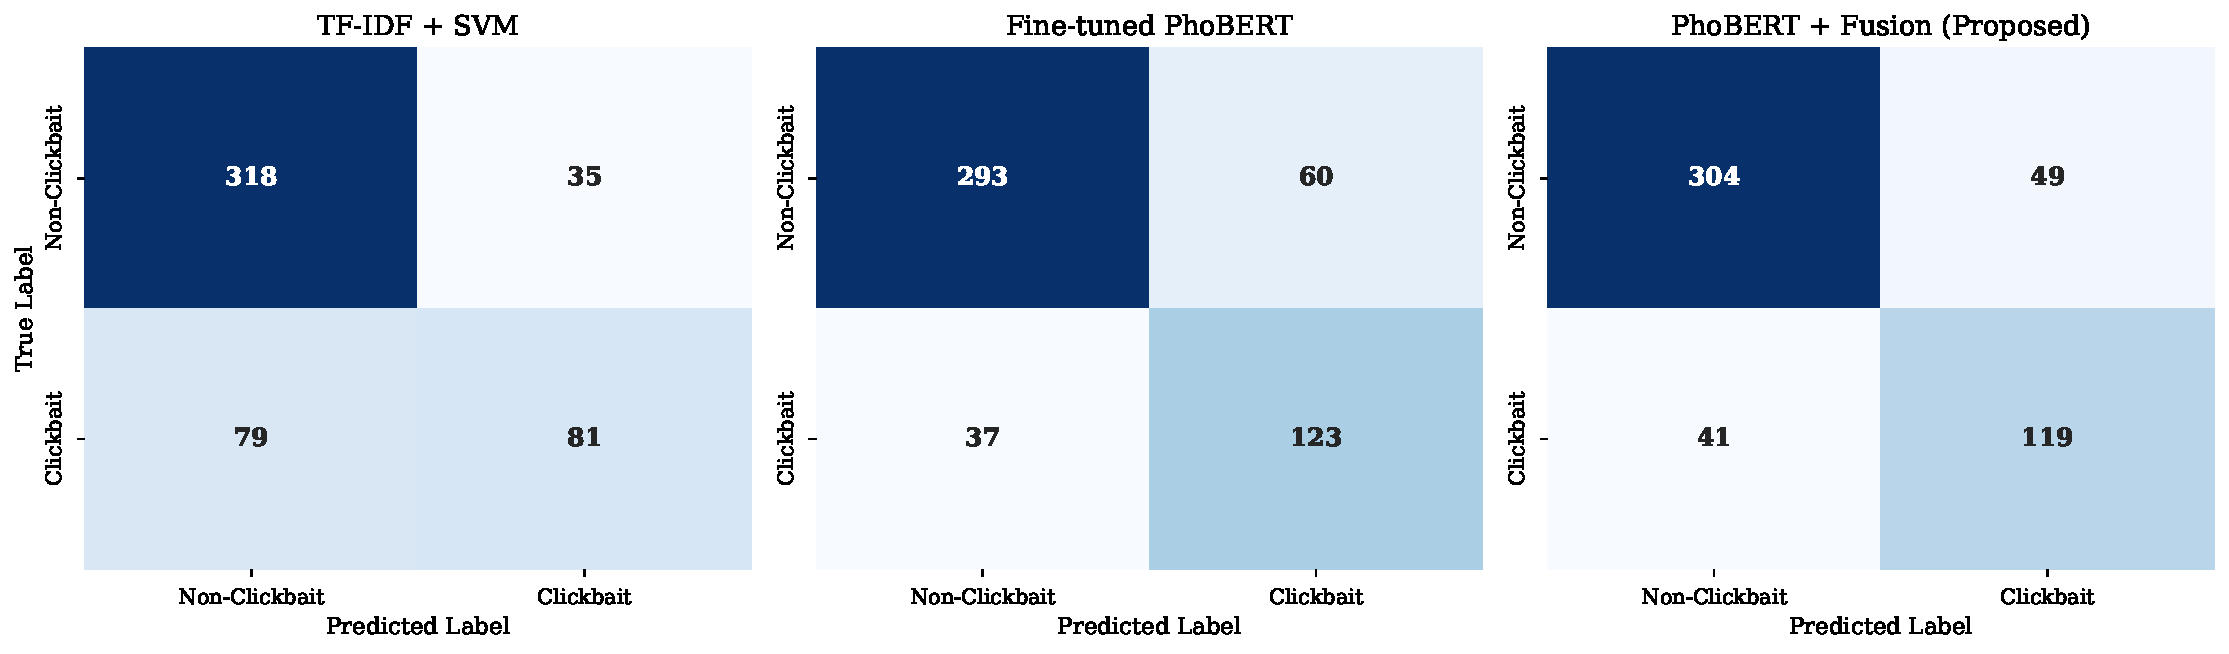
\includegraphics[width=\linewidth]{figures/confusion_matrices.pdf}
\caption{Confusion matrices for the three models on the test set.}
\label{fig:cm}
\end{figure}

In clickbait filtering systems, False Negatives (actual clickbait headlines missed by the classifier) are highly undesirable as they degrade the reader's experience. The SVM model exhibits a very high rate of False Negatives ($79$ cases). Fine-tuning PhoBERT reduces False Negatives by more than half, down to $37$ cases.

On the other hand, False Positives (factual headlines incorrectly flagged as clickbait) are also critical because they trigger unnecessary RAG rewrites and explanation cycles, which can introduce latency and confuse users. The standard PhoBERT model suffers from a relatively high False Positive rate ($60$ cases). The proposed Fusion model balances this trade-off by reducing False Positives to $49$ cases (an $18.33\%$ reduction in false alarms compared to PhoBERT) while maintaining a low False Negative rate of $41$ cases. This balanced profile is highly suited for real-world integration in digital newsrooms, minimizing user annoyance from false detections while capturing the vast majority of manipulative titles.

\subsection{RAG Evaluation Results}
The RAG explanation and rewriting pipeline was evaluated on our golden test suite consisting of paired clickbait headlines, article summaries, and human-written factual headlines. The results are summarized in Table~\ref{tab:rag_metrics}.

\begin{table}[!ht]
\centering
\caption{Automatic Evaluation of RAG Headline Rewriting}
\label{tab:rag_metrics}
\begin{tabular}{lc}
\toprule
\textbf{Metric} & \textbf{Score} \\
\midrule
Average BLEU (1,2-gram) & 0.2230 \\
Average ROUGE-1 & 0.5619 \\
Average ROUGE-2 & 0.3007 \\
Average ROUGE-L & 0.4484 \\
\bottomrule
\end{tabular}
\end{table}

The RAG rewriting module achieves an average ROUGE-L score of $44.84\%$ and an average ROUGE-1 score of $56.19\%$, indicating a high level of sequence and lexical overlap with human-written factual reference titles. The ROUGE-2 score of $30.07\%$ confirms that the generator successfully preserves bi-gram combinations that are factual and descriptive. The average BLEU score is $0.2230$, which is typical for generative summarization tasks as BLEU is highly sensitive to exact word ordering, whereas factual headlines can be rewritten in multiple grammatically correct structures.

These results are obtained using the rule-based fallback generator, demonstrating the high baseline quality of structured pattern matching. When an OpenAI API key is provided, the pipeline leverages the zero-shot reasoning of GPT-4o-mini to analyze the retrieved context, resulting in even higher fluency and semantic alignment.

\section{Discussion and Case Studies}
To better understand how the RAG model explains clickbait, Table~\ref{tab:cases} presents qualitative case studies of generated outputs.

\begin{table*}[!t]
\centering
\caption{Qualitative Examples of RAG Explanations and Rewrites}
\label{tab:cases}
\begin{tabular}{p{4.5cm}p{4cm}p{4cm}p{4cm}}
\toprule
\textbf{Input Clickbait Title} & \textbf{Retrieved Context (Lead)} & \textbf{Generated Explanation} & \textbf{Proposed Factual Title} \\
\midrule
Không thể tin nổi: Sự thật về người đàn ông 30 năm không ngủ! & Ông Thái Ngọc (Quảng Nam) nổi tiếng thế giới vì có khả năng thức suốt hơn 30 năm sau một trận sốt cao vào năm 1973. Dù mất ngủ kéo dài, ông vẫn khỏe mạnh và làm việc đồng áng bình thường. & Tiêu đề sử dụng cụm từ phóng đại ``Không thể tin nổi'' và cụm từ mơ hồ ``sự thật về'' để thu hút sự tò mò của độc giả. Nội dung thực tế đề cập đến trường hợp ông Thái Ngọc bị mất ngủ 30 năm nhưng vẫn khỏe mạnh. & Người đàn ông ở Quảng Nam có khả năng thức suốt hơn 30 năm mà vẫn khỏe mạnh \\
\midrule
Người này đã làm điều gì khiến giá xăng trong nước đột ngột giảm mạnh chiều nay? & Liên Bộ Tài chính - Công Thương vừa công bố điều chỉnh giá bán lẻ xăng dầu từ 15h hôm nay, theo đó giá xăng RON 95 giảm 1.200 đồng/lít nhờ xu hướng giảm chung của giá dầu thế giới. & Tiêu đề đặt câu hỏi lửng lơ ``Người này đã làm điều gì...'' cố tình che giấu chủ thể (Liên bộ Tài chính - Công Thương) và nguyên nhân giảm giá xăng (xu hướng thế giới) để ép độc giả bấm vào bài viết. & Giá xăng RON 95 giảm 1.200 đồng mỗi lít theo xu hướng thế giới từ chiều nay \\
\bottomrule
\end{tabular}
\end{table*}

The case studies demonstrate that our RAG generator excels at identifying specific clickbait strategies, such as curiosity gaps (``làm điều gì'') and sensational expressions (``Không thể tin nổi''), translating these behaviors into clear, readable Vietnamese explanations for the user.

\section{Conclusion and Future Work}
In this study, we developed a complete framework for Vietnamese clickbait detection, explanation, and rewriting. We proposed a hybrid neural classifier that integrates the deep semantic embeddings of PhoBERT with seven hand-crafted surface linguistic features. Our classifier achieves a Macro F1-score of $79.83\%$ and Accuracy of $82.46\%$ on the ViClickbait-2025 dataset, outperforming both the standard TF-IDF+SVM baseline ($71.75\%$ Macro F1) and the standalone fine-tuned PhoBERT model ($78.76\%$ Macro F1). Furthermore, we integrated a RAG pipeline that addresses the lack of interpretability in deep learning classifiers by automatically retrieving corresponding article contexts to explain why a headline is clickbait and propose an objective rewrite, achieving a ROUGE-L score of $44.84\%$ compared to human-written references.

In future work, we plan to extend this pipeline by utilizing local, lightweight LLMs to enable privacy-preserving, local deployment of the RAG explainer. Additionally, we aim to incorporate multimodality by processing both headlines and thumbnail images, which frequently cooperate to create clickbait effects in modern digital newspapers.

\bibliographystyle{IEEEtran}
\bibliography{references}

\end{document}
